% $Id: template.tex 11 2007-04-03 22:25:53Z jpeltier $


\documentclass{vgtc}                          % final (conference style)
%\documentclass[review]{vgtc}                 % review
%\documentclass[widereview]{vgtc}             % wide-spaced review
%\documentclass[preprint]{vgtc}               % preprint
%\documentclass[electronic]{vgtc}             % electronic version

\makeatletter
\let\@citex\asme@citex % restore
\makeatother

%% Uncomment one of the lines above depending on where your paper is
%% in the conference process. ``review'' and ``widereview'' are for review
%% submission, ``preprint'' is for pre-publication, and the final version
%% doesn't use a specific qualifier. Further, ``electronic'' includes
%% hyperreferences for more convenient online viewing.

%% Please use one of the ``review'' options in combination with the
%% assigned online id (see below) ONLY if your paper uses a double blind
%% review process. Some conferences, like IEEE Vis and InfoVis, have NOT
%% in the past.

%% Figures should be in CMYK or Grey scale format, otherwise, colour 
%% shifting may occur during the printing process.

%% These few lines make a distinction between latex and pdflatex calls and they
%% bring in essential packages for graphics and font handling.
%% Note that due to the \DeclareGraphicsExtensions{} call it is no longer necessary
%% to provide the the path and extension of a graphics file:
%% 
\includegraphics{diamondrule} is completely sufficient.
%%
\ifpdf%                                % if we use pdflatex
  \pdfoutput=1\relax                   % create PDFs from pdfLaTeX
  \pdfcompresslevel=9                  % PDF Compression
  \pdfoptionpdfminorversion=7          % create PDF 1.7
  \ExecuteOptions{pdftex}
  \usepackage{graphicx}                % allow us to embed graphics files	
  \DeclareGraphicsExtensions{.pdf,.png,.jpg,.jpeg} % for pdflatex we expect .pdf, .png, or .jpg files
\else%                                 % else we use pure latex
  \ExecuteOptions{dvips}
  \usepackage{graphicx}                % allow us to embed graphics files
  \DeclareGraphicsExtensions{.eps}     % for pure latex we expect eps files
\fi%

%% it is recomended to use ``\autoref{sec:bla}'' instead of ``Fig.~\ref{sec:bla}''
\graphicspath{size_and_scatterplots_files/figure-latex} % where to search for the images

\usepackage{microtype}                 % use micro-typography (slightly more compact, better to read)
\PassOptionsToPackage{warn}{textcomp}  % to address font issues with \textrightarrow
\usepackage{textcomp}                  % use better special symbols
\usepackage{mathptmx}                  % use matching math font
\usepackage{times}
\usepackage[T1]{fontenc}               % we use Times as the main font
\renewcommand*\ttdefault{txtt}         % a nicer typewriter font
\usepackage{cite}                      % needed to automatically sort the references
\usepackage{tabu}                      % only used for the table example
\usepackage{booktabs}                  % only used for the table example
%% We encourage the use of mathptmx for consistent usage of times font
%% throughout the proceedings. However, if you encounter conflicts
%% with other math-related packages, you may want to disable it.


%% If you are submitting a paper to a conference for review with a double
%% blind reviewing process, please replace the value ``0'' below with your
%% OnlineID. Otherwise, you may safely leave it at ``0''.
\onlineid{0}

%% declare the category of your paper, only shown in review mode
\vgtccategory{Research}

%% allow for this line if you want the electronic option to work properly
\vgtcinsertpkg

%% In preprint mode you may define your own headline. If not, the default IEEE copyright message will appear in preprint mode.
%\preprinttext{To appear in an IEEE VGTC sponsored conference.}

%% This adds a link to the version of the paper on IEEEXplore
%% Uncomment this line when you produce a preprint version of the article 
%% after the article receives a DOI for the paper from IEEE
%\ieeedoi{xx.xxxx/TVCG.201x.xxxxxxx}


%% Paper title.

\title{Point Size and Correlation Perception in Scatterplots}

%% This is how authors are specified in the conference style

%% Author and Affiliation (single author).
%%\author{Roy G. Biv\thanks{e-mail: roy.g.biv@aol.com}}
%%\affiliation{\scriptsize Allied Widgets Research}

%% Author and Affiliation (multiple authors with single affiliations).
%%\author{Roy G. Biv\thanks{e-mail: roy.g.biv@aol.com} %
%%\and Ed Grimley\thanks{e-mail:ed.grimley@aol.com} %
%%\and Martha Stewart\thanks{e-mail:martha.stewart@marthastewart.com}}
%%\affiliation{\scriptsize Martha Stewart Enterprises \\ Microsoft Research}

%% Author and Affiliation (multiple authors with multiple affiliations)
\author{Gabriel Strain\thanks{\href{mailto:Gabriel.Strain@manchester.ac.uk}{\nolinkurl{Gabriel.Strain@manchester.ac.uk}}} %
\and Andrew J. Stewart\thanks{\href{mailto:Andrew.J.Stewart@manchester.ac.uk}{\nolinkurl{Andrew.J.Stewart@manchester.ac.uk}}} %
\and Paul Warren\thanks{\href{mailto:Paul.Warren@manchester.ac.uk}{\nolinkurl{Paul.Warren@manchester.ac.uk}}} %
\and Caroline Jay\thanks{\href{mailto:Caroline.Jay@manchester.ac.uk}{\nolinkurl{Caroline.Jay@manchester.ac.uk}}}} %
 \affiliation{\scriptsize The University of Manchester}


%% Abstract section.
\abstract{Place abstract here.}

%% ACM Computing Classification System (CCS). 
%% See <http://www.acm.org/about/class> for details.
%% We recommend the 2012 system <http://www.acm.org/about/class/class/2012>
%% For the 2012 system use the ``\CCScatTwelve'' which command takes four arguments.
%% The 1998 system <http://www.acm.org/about/class/class/2012> is still possible
%% For the 1998 system use the ``\CCScat'' which command takes four arguments.
%% In both cases the last two arguments (1998) or last three (2012) can be empty.

\CCScatlist{
  \CCScatTwelve{Human-centered computing}{Visu\-al\-iza\-tion}{Empirical studies in visualization};
  \CCScatTwelve{Human-centered computing}{Human computer interaction (HCI)}{Empirical studies in HCI}
}

%\CCScatlist{
  %\CCScat{H.5.2}{User Interfaces}{User Interfaces}{Graphical user interfaces (GUI)}{};
  %\CCScat{H.5.m}{Information Interfaces and Presentation}{Miscellaneous}{}{}
%}

%% Copyright space is enabled by default as required by guidelines.
%% It is disabled by the 'review' option or via the following command:
% \nocopyrightspace

%%%%%%%%%%%%%%%%%%%%%%%%%%%%%%%%%%%%%%%%%%%%%%%%%%%%%%%%%%%%%%%%
%%%%%%%%%%%%%%%%%%%%%% START OF THE PAPER %%%%%%%%%%%%%%%%%%%%%%
%%%%%%%%%%%%%%%%%%%%%%%%%%%%%%%%%%%%%%%%%%%%%%%%%%%%%%%%%%%%%%%%%

\begin{document}

%% The ``\maketitle'' command must be the first command after the
%% ``\begin{document}'' command. It prepares and prints the title block.

%% the only exception to this rule is the \firstsection command
\firstsection{}

\maketitle

\hypertarget{introduction}{%
\section{Introduction}\label{introduction}}

Scatterplots, utilised in scientific communication for a variety of tasks,
are some of the most widely used and widely studied data visualizations. Viewers
mostly interpret them in similar ways \cite{kay_heer_2015}, and they are simple
enough to be easily studied while providing important insights into visualization
design, human-computer interaction, and human perception. In a previous study \cite{strain_2023},
we showed that a novel point contrast manipulation, in which the contrast of a certain
scatterplot point was reduced as the size of that point's residual increased, could be
used to partially correct for a systematic underestimation bias present in the
literature \cite{strahan_1978, bobko_1979, cleveland_1984, lane_1985, lauer_1989, 
collyer_1990, meyer_1992}. We suggested that this was due to a narrowing of the width
of the perceived probability distribution of a particular plot brought
on by the lower contrast (and therefore lower point-salience) in those outer
areas. We tested linear, non-linear, and non-linear inverted functions relating
point contrast to residual size, finding that the non-linear function produced
the most accurate estimates of correlation, and that the non-linear inverted produced
the least accurate.

\hypertarget{scatterplots-and-correlation}{%
\subsection{Scatterplots and Correlation}\label{scatterplots-and-correlation}}

Scatterplots have been widely studied, especially as mediums for the communication
of correlation (see \cite{strain_2023} for a detailed review of this history). Much
previous work has found evidence for a pronounced underestimation in judgements
of correlation in positively correlated plots, especially between 0.2 \textless{} \emph{r} \textless{} 0.6. The
nature of this investigation has varied, ranging from direct estimation techniques,
to discriminative judgement, bisection, and staircase tasks. As in our previous work,
we choose to use the direct estimation paradigm owing to its simplicity, and its suitability
to online experimentation. The use of this paradigm renders the judgements we collect
comparative by nature, although such work does allow us to inform design guidelines as
well as human perception. It is our duty as visualization designers to ensure that the
messages we are trying to communicate are being interpreted as accurately as possible
by viewers. To do this, we must understand human perception, apply that understanding
to design, and test those designs in rigorous empirical studies.

\hypertarget{point-size}{%
\subsection{Point Size}\label{point-size}}

Point contrast is not the only available visual feature that might be used
to influence viewer's perceptions of the width of a probability distribution. Nor is
it the only visual feature of a scatterplot that we can exploit. While
contrast adjustments have been used extensively to solve issues of overplotting and clutter
in scatterplots \cite{matejka_2015, bertini_2004}, there is no established use for
varying point size. Common sense dictates that scatterplots visualizing larger
datasets inherently require their points to be smaller to prevent the obscuring of data,
but to our knowledge there is little testing of impact of point size on correlation perception.
Studies have found invariance in in the bias and variability of correlation
estimation with regards to changing point sizes \cite{rensink_2012, rensink_2014},
but these have been low-powered. From the wider literature there is evidence that larger points
are more salient \cite{healey_2012}, can bias judgements of point position
\cite{hong_2021}, and can result in faster reaction times \cite{grice_1983} to
peripherally presented stimuli. In addition, smaller stimuli are associated with
greater levels of spatial uncertainty \cite{alais_2004}, and if this
is driving the reduction in error we saw in our previous work \cite{strain_2023},
we would expect a similar effect when point size is used instead of point contrast.

\hypertarget{hypotheses}{%
\subsection{Hypotheses}\label{hypotheses}}

We hypothesize that correlation estimation will be most accurate when
viewers are presented with the non-linear size decay condition, and will be
least accurate when presented with the non-linear inverted size decay condition.
We thereby present a single experiment study in which we demonstrate that the use of
a non-linear size decay function relating to the residuals of points on scatterplots
can be employed to correct for a systematic underestimation of correlation by
viewers in scatterplots. We find no evidence for an effect of graph literacy (put
something about training here). The effect we observe here is much stronger, both
with regards to effect size and in terms of the observed reduction in error, than the
effect we observed in our previous study \cite{strain_2023}. We suggest that this
function can be used to facilitate more accurate correlation
perception in scatterplots, and provide exciting future avenues for the continuation
and refinement of these techniques. Ethical approval was granted by the University
of Manchester's Computer Science Departmental Panel (Ref: 2022-14660-24397).

\hypertarget{methodology}{%
\section{Methodology}\label{methodology}}

\hypertarget{open-research-statement}{%
\subsection{Open Research Statement}\label{open-research-statement}}

The experiment was conducted according to the principles of open and reproducible research.
All data and analysis code are available at \url{https://github.com/gjpstrain/size_and_scatterplots}.
This repository contains instructions for building a docker image to fully
reproduce the computational environment used, allowing for full replications
of stimulus generation, analyses, and the paper itself. The experiment was
pre-registered with the OSF (\url{https://osf.io/k4gd8}).

\hypertarget{participants}{%
\subsection{Participants}\label{participants}}

150 participants were recruited using the Prolific.co platform. Normal to
corrected-to-normal vision and English fluency were required for participation. As in
\cite{strain_2023}, and in accordance with previously published guidelines \cite{peer_2021},
participants were required to have completed at least 100 studies on Prolific, and were
required to have a Prolific score of at least 100, indicating acceptance on at least
100/101 previously completed studies. Participants who took part in any of our
previous studies were prevented from participating, and participants were only
permitted to complete the experiment on a desktop or laptop computer.

Data were collected from 164 participants. 14 failed more than 2 out of 6 attention
check questions, and, as per pre-registration stipulations, were rejected from the study. Data
from 150 participants was included in the analysis (48.00\% male, 50.00\% female, and 2\% non-binary). Mean age of participants was 29.56
(\emph{SD} = 8.54). Mean graph literacy score was 21.77
(\emph{SD} = 4.29) out of 30. The average time taken to complete
the experiment was 39 minutes (SD = 14 minutes).

\hypertarget{stimuli}{%
\subsection{Stimuli}\label{stimuli}}

The data used to generated the scatterplots in the current study was identical to that
used previously \cite{strain_2023}. Scatterplots were generated based on 45 uniformly distributed \emph{r} values
between 0.2 and 0.99. Scatterplot points were generated based on bivariate normal
distributions with standard deviations of 1 in each direction. Each scatterplot
had a 1:1 aspect ratio, was generated as a 1200 x 1200 pixel .png image, and was
scaled up or down according to the participant's monitor. See \autoref{dot-pitch-and-crowdsourced-experiments}
for a more detailed discussion of precise point sizes and dot pitch in crowd-sourced
experiments.

As in our previous study \cite{strain_2023}, we used equation 1 to map residuals
to point sizes in three of our conditions. We used a scaling factor of 4 and a constant of 0.2 to achieve a
minimum point size of 12/13 pixels, which is consistent with the point size on
a 1920 x 1080 monitor for both experiments in \cite{strain_2023}. Again, see \autoref{dot-pitch-and-crowdsourced-experiments} for a discussion of dot pitch.
In our fourth condition, which we refer to as ``Standard size'', point size was uniformly
set to be consistent with the point size in our previous studies.
Scripts detailing scatterplot and mask generation can be found in the item
preparation folder in the repository linked below.

\begin{equation}
  point-size = 1 - b^R
\end{equation}

\hypertarget{dot-pitch-and-crowdsourced-experiments}{%
\subsection{Dot Pitch and Crowdsourced Experiments}\label{dot-pitch-and-crowdsourced-experiments}}

In our previous study \cite{strain_2023}, we had no way of obtaining dot pitch
or participant to monitor distance due to the online, crowdsourced nature of the
experiments. Since then we have adopted a method for obtaining the height of a
participant's monitor in inches \cite{screenscale}. Combining this with the
monitor resolution fetched from Psychopy and assuming a widescreen 16:9 aspect ratio
allows us to infer dot pitch and therefore the physical size of the points in our
experiment. Mean dot pitch was 0.33mm, (\(SD = 0.06\)),
corresponding to a physical size on the screen of 4.32mm
for the smallest points displayed. While dot pitch is not necessary information for the present study, as we are only
interested in the relative differences in correlation estimates between point size
conditions, the fact that we can collect it at all is indicative of the gap
being narrowed with regards to psychophysical testing between in-person and online
experiments. Given that the latter are cheaper, easier, and immeasurably quicker,
anything that can be done be done to narrow this gap in capability is a boon.
See \autoref{results} for analyses including dot pitch as a predictor.

\hypertarget{visual-threshold-testing}{%
\subsection{Visual Threshold Testing}\label{visual-threshold-testing}}

It is key that our manipulation does not functionally removing data from the scatterplot,
thus, in order to test that all our points were visible across a range of viewing
contexts and on a range of apparatus, we included visual threshold testing prior
to the experimental items in the study. Participants were shown six scatterplots
with a number of points, and were asked to enter in a textbox how many points
were being displayed. The points were the same size as the smallest points used
in the experimental materials. 5\% of
participants were correct on 5 out of 6 visual
threshold questions, while 95\% were correct
on 6 out of 6. It should be noted that those
participants scoring 5/6 did not answer incorrectly, rather did not answer
at all for this particular questions, which is more suggestive of either
a mis-click or an initial misunderstanding of the task they were asked to complete.
Regardless, we consider these results to be indicative of a sufficient level of
point visibility for the current experiment.

\hypertarget{design}{%
\subsection{Design}\label{design}}

The experiment used a fully repeated measures, within-participants design, with each
participant seeing and responding to each of the 180 scatterplots in a randomised order.
There were four scatterplots for each of the 45 \emph{r} values corresponding to the
four levels of the size condition, examples of which can be see in Figure \ref{fig:examples}.
Everything needed to run the experiment, including code, materials, instructions, and scripts, is
hosted at \url{https://gitlab.pavlovia.org/Strain/exp_size_only}.

\begin{figure}
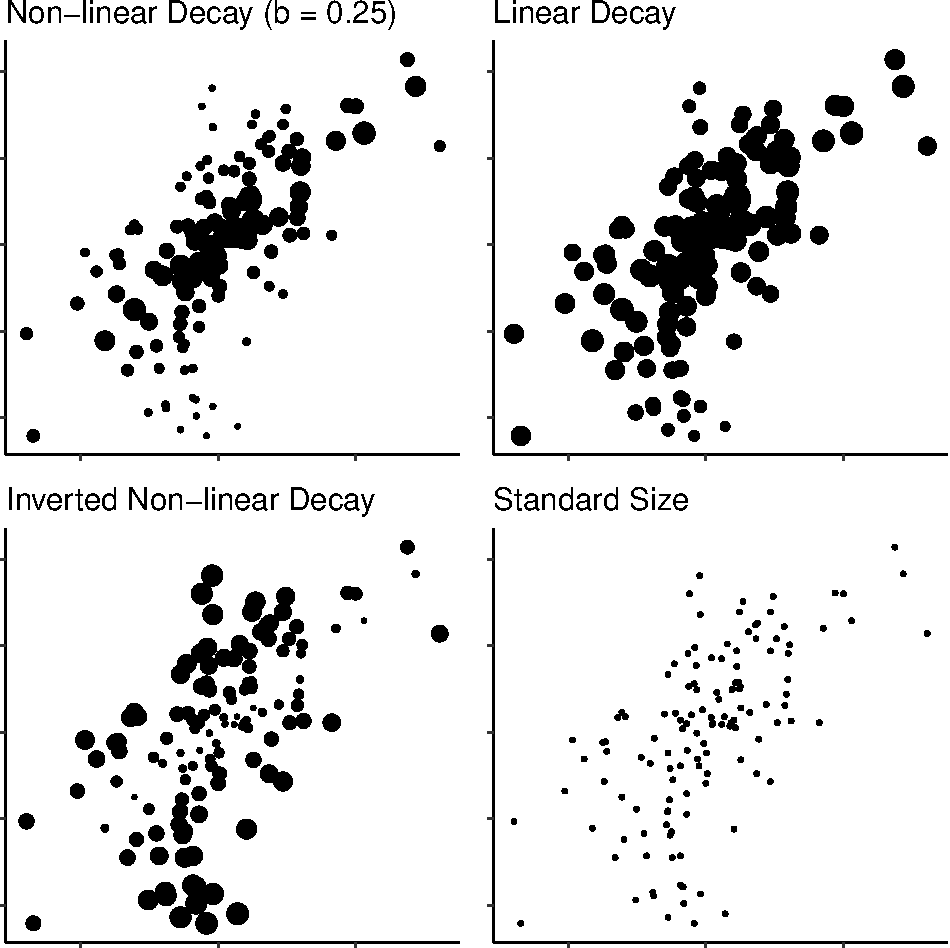
\includegraphics[width=1\linewidth]{size_and_scatterplots_files/figure-latex/examples-1} \caption{Four levels of the point size condition, demonstrated with an \textit{r} value of 0.6}\label{fig:examples}
\end{figure}

\hypertarget{procedure}{%
\subsection{Procedure}\label{procedure}}

Each participants was shown the participants information sheet (PIS) and provided
consent through key presses in response to consent statements. They were asked
to provide their age in a free text box, and their gender identity. Participants
then completed the 5-item Subjective Graph Literacy (SGL) test \cite{garcia_2016},
followed by the visual threshold testing described above. Participants then completed
the screen scaling task described in \autoref{dot-pitch-and-crowdsourced-experiments}.
Participants were given instructions, and then shown examples of \emph{r} = 0.2, 0.5, 0.8, and
0.95, as in our previous work \cite{strain_2023}. \autoref{training} includes
a discussion of the potential effects of this training. Two practice trials were
given before the experiment began. Participants worked through a series of 180 trials
in which they were asked to use a slider to estimate the correlation shown in
the scatterplot. Visual masks preceded each plot. Interspersed were six attention check trials which asked
participants to set the slider to 1 or 0 and ignore the scatterplot.

\hypertarget{results}{%
\section{Results}\label{results}}

All analyses were conducted using R (version 4.2.3 \cite{r_core}). Models were
built using the \textbf{buildmer} (version 2.8 \cite{voeten_buildmer_2022}) and \textbf{lme4}
(version 1.1-32 \cite{bates_lme4_2015}) packages, with size manipulation being set
as the predictor for participants' errors in correlation estimates

\begin{figure}
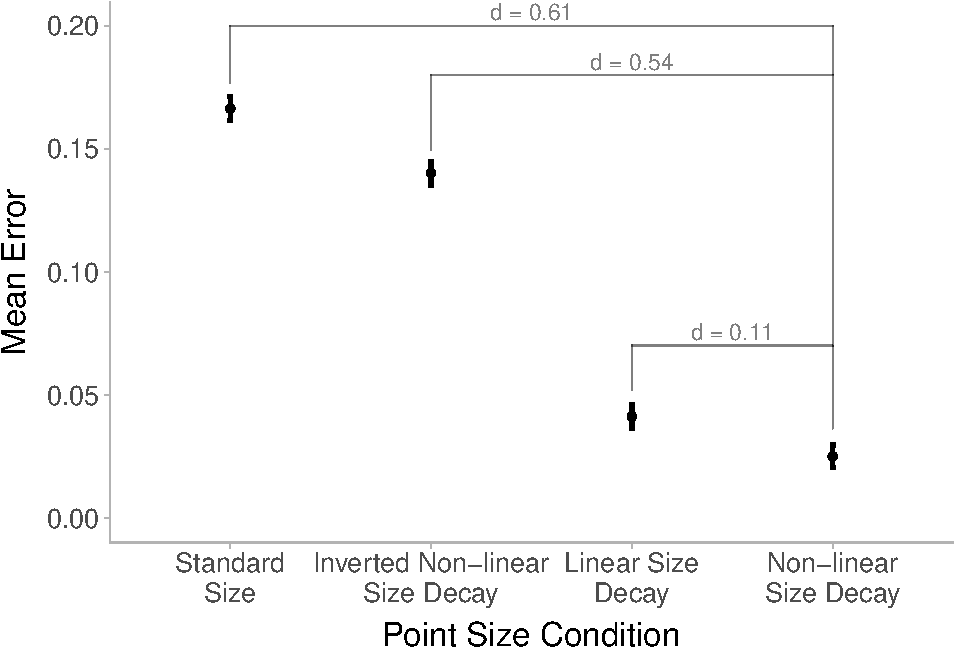
\includegraphics[width=1\linewidth]{size_and_scatterplots_files/figure-latex/dot-plot-1} \caption{Mean error in correlation estimates across the four size manipulation conditions, with 95\% confidence intervals shown. Brackets show the effect sizes between standard size and all other conditions in Cohen's d.}\label{fig:dot-plot}
\end{figure}

Mean errors in correlation estimates for the four size manipulation conditions
can be seen in figure \ref{fig:dot-plot}. A likelihood ratio test revealed that the
model including size manipulation as a predictor explained significantly more
variance than a null model (\(\chi^2\)(3) = 3,508.84,
\emph{p} \textless{} .001). This model has random intercepts for
items and participants. The effect here is driven by participants' errors being lower
for scatterplots with the non-linear size decay manipulation than for all other conditions,
for error being lower for scatterplots with linear size decay than for plots with
inverted non-linear decay or standard size, and for errors being higher for scatterplots
with standard size than for plots with inverted non-linear decay.

Testing for contrasts between the four levels of the size manipulation condition
were performed with the \textbf{emmeans} package (version 1.8.5 \cite{emmeans}), and
of correlation estimates are shown in Figure \ref{fig:dot-plot}. The \textbf{EMAtools} package
was used to calculate effects sizes in Cohen's d, the results of which can be seen in
\ref{fig:dot-plot}. The largest effect size we found was 0.61 when comparing
the non-linear size decay and standard size conditions. This is significantly higher
than any of the effects sizes we have found in our previous work.

\begin{table}

\caption{\label{tab:contrasts-table}Contrasts between each of the four levels of the size decay condition.}
\centering
\resizebox{\linewidth}{!}{
\begin{tabular}[t]{lrl}
\toprule
Contrast & Z.ratio & p.value\\
\midrule
Standard Size : Inverted Non-linear Decay & 9.35 & <0.001\\
Standard Size : Non-linear Decay & 50.14 & <0.001\\
Standard Size : Linear Decay & 44.40 & <0.001\\
Inverted Non-linear Decay : Non-linear Decay & 40.79 & <0.001\\
Inverted Non-linear Decay : Linear Decay & 35.06 & <0.001\\
\addlinespace
Non-linear Decay: Linear Decay & -5.73 & <0.001\\
\bottomrule
\end{tabular}}
\end{table}

In addition, we find no significant difference between the experimental model
and another including graph literacy as a fixed effect (\(\chi^2\)(1)
0.16, \emph{p} = .690),
suggesting the effect we found was not driven by differences in graph literacy.

\begin{figure*}

{\centering 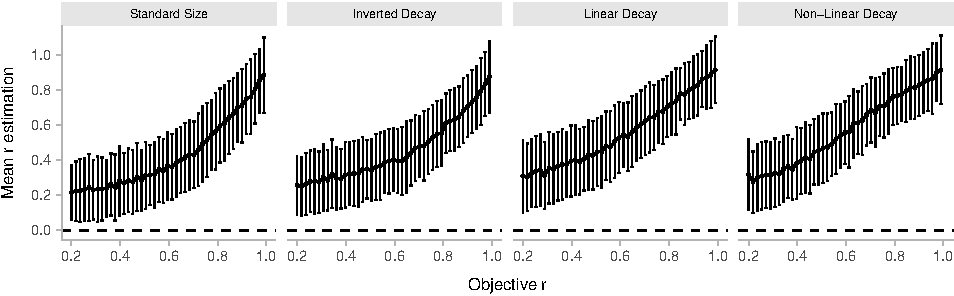
\includegraphics[width=1\linewidth]{size_and_scatterplots_files/figure-latex/error-plot-1} 

}

\caption{hello2}\label{fig:error-plot}
\end{figure*}

\begin{figure*}

{\centering 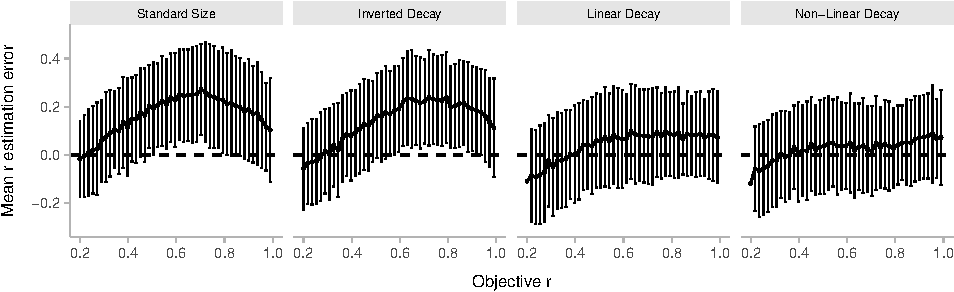
\includegraphics[width=1\linewidth]{size_and_scatterplots_files/figure-latex/changes-with-r-size-1} 

}

\caption{hello}\label{fig:changes-with-r-size}
\end{figure*}

Figure \ref{fig:changes-with-r-size} shows how participants' mean errors in correlation
estimates change with the objective Pearson's \emph{r} value, plotted separately for each
size decay condition. Note the close-to-zero errors present in the non-linear size
decay condition.

As discussed previously, in the present study we employed a method for obtaining
a measurement of dot pitch from each participant. While \ref{visual-threshold-testing}
provides evidence that participants had little to no problem perceiving all the dots
on the scatterplots shown, there may be some other facet of using a larger or smaller
monitor with a larger or smaller resolution that could have affected the estimates
our participants gave. To check this, we built a model including the dot pitch
measurement as a fixed effect. Comparing this to the experimental model revealed
no significant effect of dot pitch (\(\chi^2\)(1) = 4.65, \emph{p} = .031)

\hypertarget{discussion}{%
\section{Discussion}\label{discussion}}

We found support for our first hypothesis. As can be seen in \ref{fig:changes-with-r-size},
participants' errors in correlation estimation were significantly lower when
they were presented with the non-linear size decay condition (see \ref{fig:examples})
compared to when they were presented with all other conditions. We found no support
for our second hypothesis, that participants' estimations would be worse in the
inverted non-linear size decay condition than all other conditions. We found that
errors in this condition were indeed significantly higher than for the other
two size decay conditions, but that this error was similar to, but significantly lower than,
the error with the standard size.

\hypertarget{training}{%
\subsection{Training}\label{training}}

%% if specified like this the section will be committed in review mode
\acknowledgments{This work was supported by funding from the University of Manchester Department of Computer Science and Division of Psychology, Communication and Human Neuroscience}

%\bibliographystyle{abbrv}
\bibliographystyle{bib_styles/abbrv-doi}
%\bibliographystyle{abbrv-doi-narrow}
%\bibliographystyle{abbrv-doi-hyperref}
%\bibliographystyle{abbrv-doi-hyperref-narrow}

\bibliography{size-and-scatterplots}
\end{document}
